\documentclass[]{article}
\usepackage[utf8]{inputenc}
\usepackage[spanish]{babel}
\usepackage{graphicx}	%Si se quiere compilar con las imagenes
\usepackage{graphics, float, fancyhdr, titling, caption, subcaption}
\usepackage{listings, xcolor}
\usepackage[a4paper, total={6in, 9.5in}]{geometry}
\usepackage{fancyhdr}
\usepackage{hyperref}		% solo se debe usar si se quiere usar \hypersetup
\usepackage{xurl}


% \usepackage{amsmath}      % Si se quiere usar \text{texto} dentro del modo matematico
%\setcounter{secnumdepth}{-2}       %Poner solo esto si no se quieren numero delante de las secciones y niveles inferiores.

\renewcommand{\footrulewidth}{0.4pt}
\title{

\includegraphics[width=1.75in]{imagenes/UGR-Logo.png} \\
\vspace*{1in}
\textbf{Cuestiones Tema 5} \\
Animación por Ordenador \\
\vspace*{0.5in}}
\author{Andrés Merlo Trujillo \\
andresmerlo@correo.ugr.es \\
77147239H \\ 
\vspace*{0.5in} \\
E.T.S. de Ingenierías Informática y de Telecomunicación \\
\textbf{Universidad de Granada}} \date{\today}

\hypersetup{
    colorlinks=true,
    linkcolor=black,
    citecolor=black
}

\renewcommand\maketitlehooka{\null\mbox{}\vfill}
\renewcommand\maketitlehookd{\vfill\null}

\definecolor{codegreen}{rgb}{0,0.6,0}
\definecolor{codegray}{rgb}{0.5,0.5,0.5}
\definecolor{codepurple}{rgb}{0.58,0,0.82}
\definecolor{backcolour}{rgb}{0.95,0.95,0.92}

\lstdefinestyle{mystyle}{
    backgroundcolor=\color{backcolour},   
    commentstyle=\color{codegreen},
    keywordstyle=\color{magenta},
    numberstyle=\tiny\color{codegray},
    stringstyle=\color{codepurple},
    basicstyle=\ttfamily\footnotesize,
    breakatwhitespace=false,         
    breaklines=true,                 
    captionpos=b,                    
    keepspaces=true,                 
    numbers=left,                    
    numbersep=5pt,                  
    showspaces=false,                
    showstringspaces=false,
    showtabs=false,                  
    tabsize=2
}

\lstset{style=mystyle}

\lstdefinelanguage{MaxScript}{
  keywords={break, case, catch, collect, continue, coordsys, default, do, else, exit, false, for, fn, global, if, in, local, macroScript, not, of, on, plugin, return, rollouts, silent, struct, then, to, true, try, undo, utilities, when, while, quat, rotate},
  keywordstyle=\color{blue}\bfseries,
%   ndkeywords={!=, #, #_, ##, %, &amp;, \&, \&, *, **, +, -, /, //, :, &lt;&lt;, &gt;&gt;, &lt;=, &gt;=, ==, ^, ~, ~=, +=, -=, *=, /=, //=, ^=, &=, &lt;&lt;=, &gt;&gt;=},
%   ndkeywordstyle=\color{red}\bfseries,
  identifierstyle=\color{black},
  sensitive=true,
  comment=[l]{--},
  morecomment=[s]{/*}{*/},
  commentstyle=\color{codegreen}\ttfamily,
  stringstyle=\color{purple}\ttfamily,
  morestring=[b]',
  morestring=[b]"
}


\usepackage{enumitem, changepage}
   
\begin{document}
\begin{titlingpage}
\maketitle
\end{titlingpage}

\tableofcontents

\newpage

\pagestyle{fancy}   %a partir de comienza el header (se salta el indice y portada)
\fancyhead[L]{Andrés Merlo Trujillo}
\fancyhead[R]{Animación por Ordenador}
%\section{Ejercicio 1}
%\begin{figure}[H]
%    \centering
%    \includegraphics[width=\textwidth]{imagenes/passwdfile.png}
%    \vspace{10pt}
%    \footnotesize{Fuente: https://...}
%\end{figure}

% \begin{figure}[H]\ContinuedFloat		% si se parten las imagenes en dos paginas y se desea continuar las letras de las subfiguras (a, b, c, ..., otra pag -> c, d, e)
% \begin{figure}[H]
%     \centering 
% 	\begin{subfigure}[t]{0.48\textwidth}
% 	    \centering
% 	    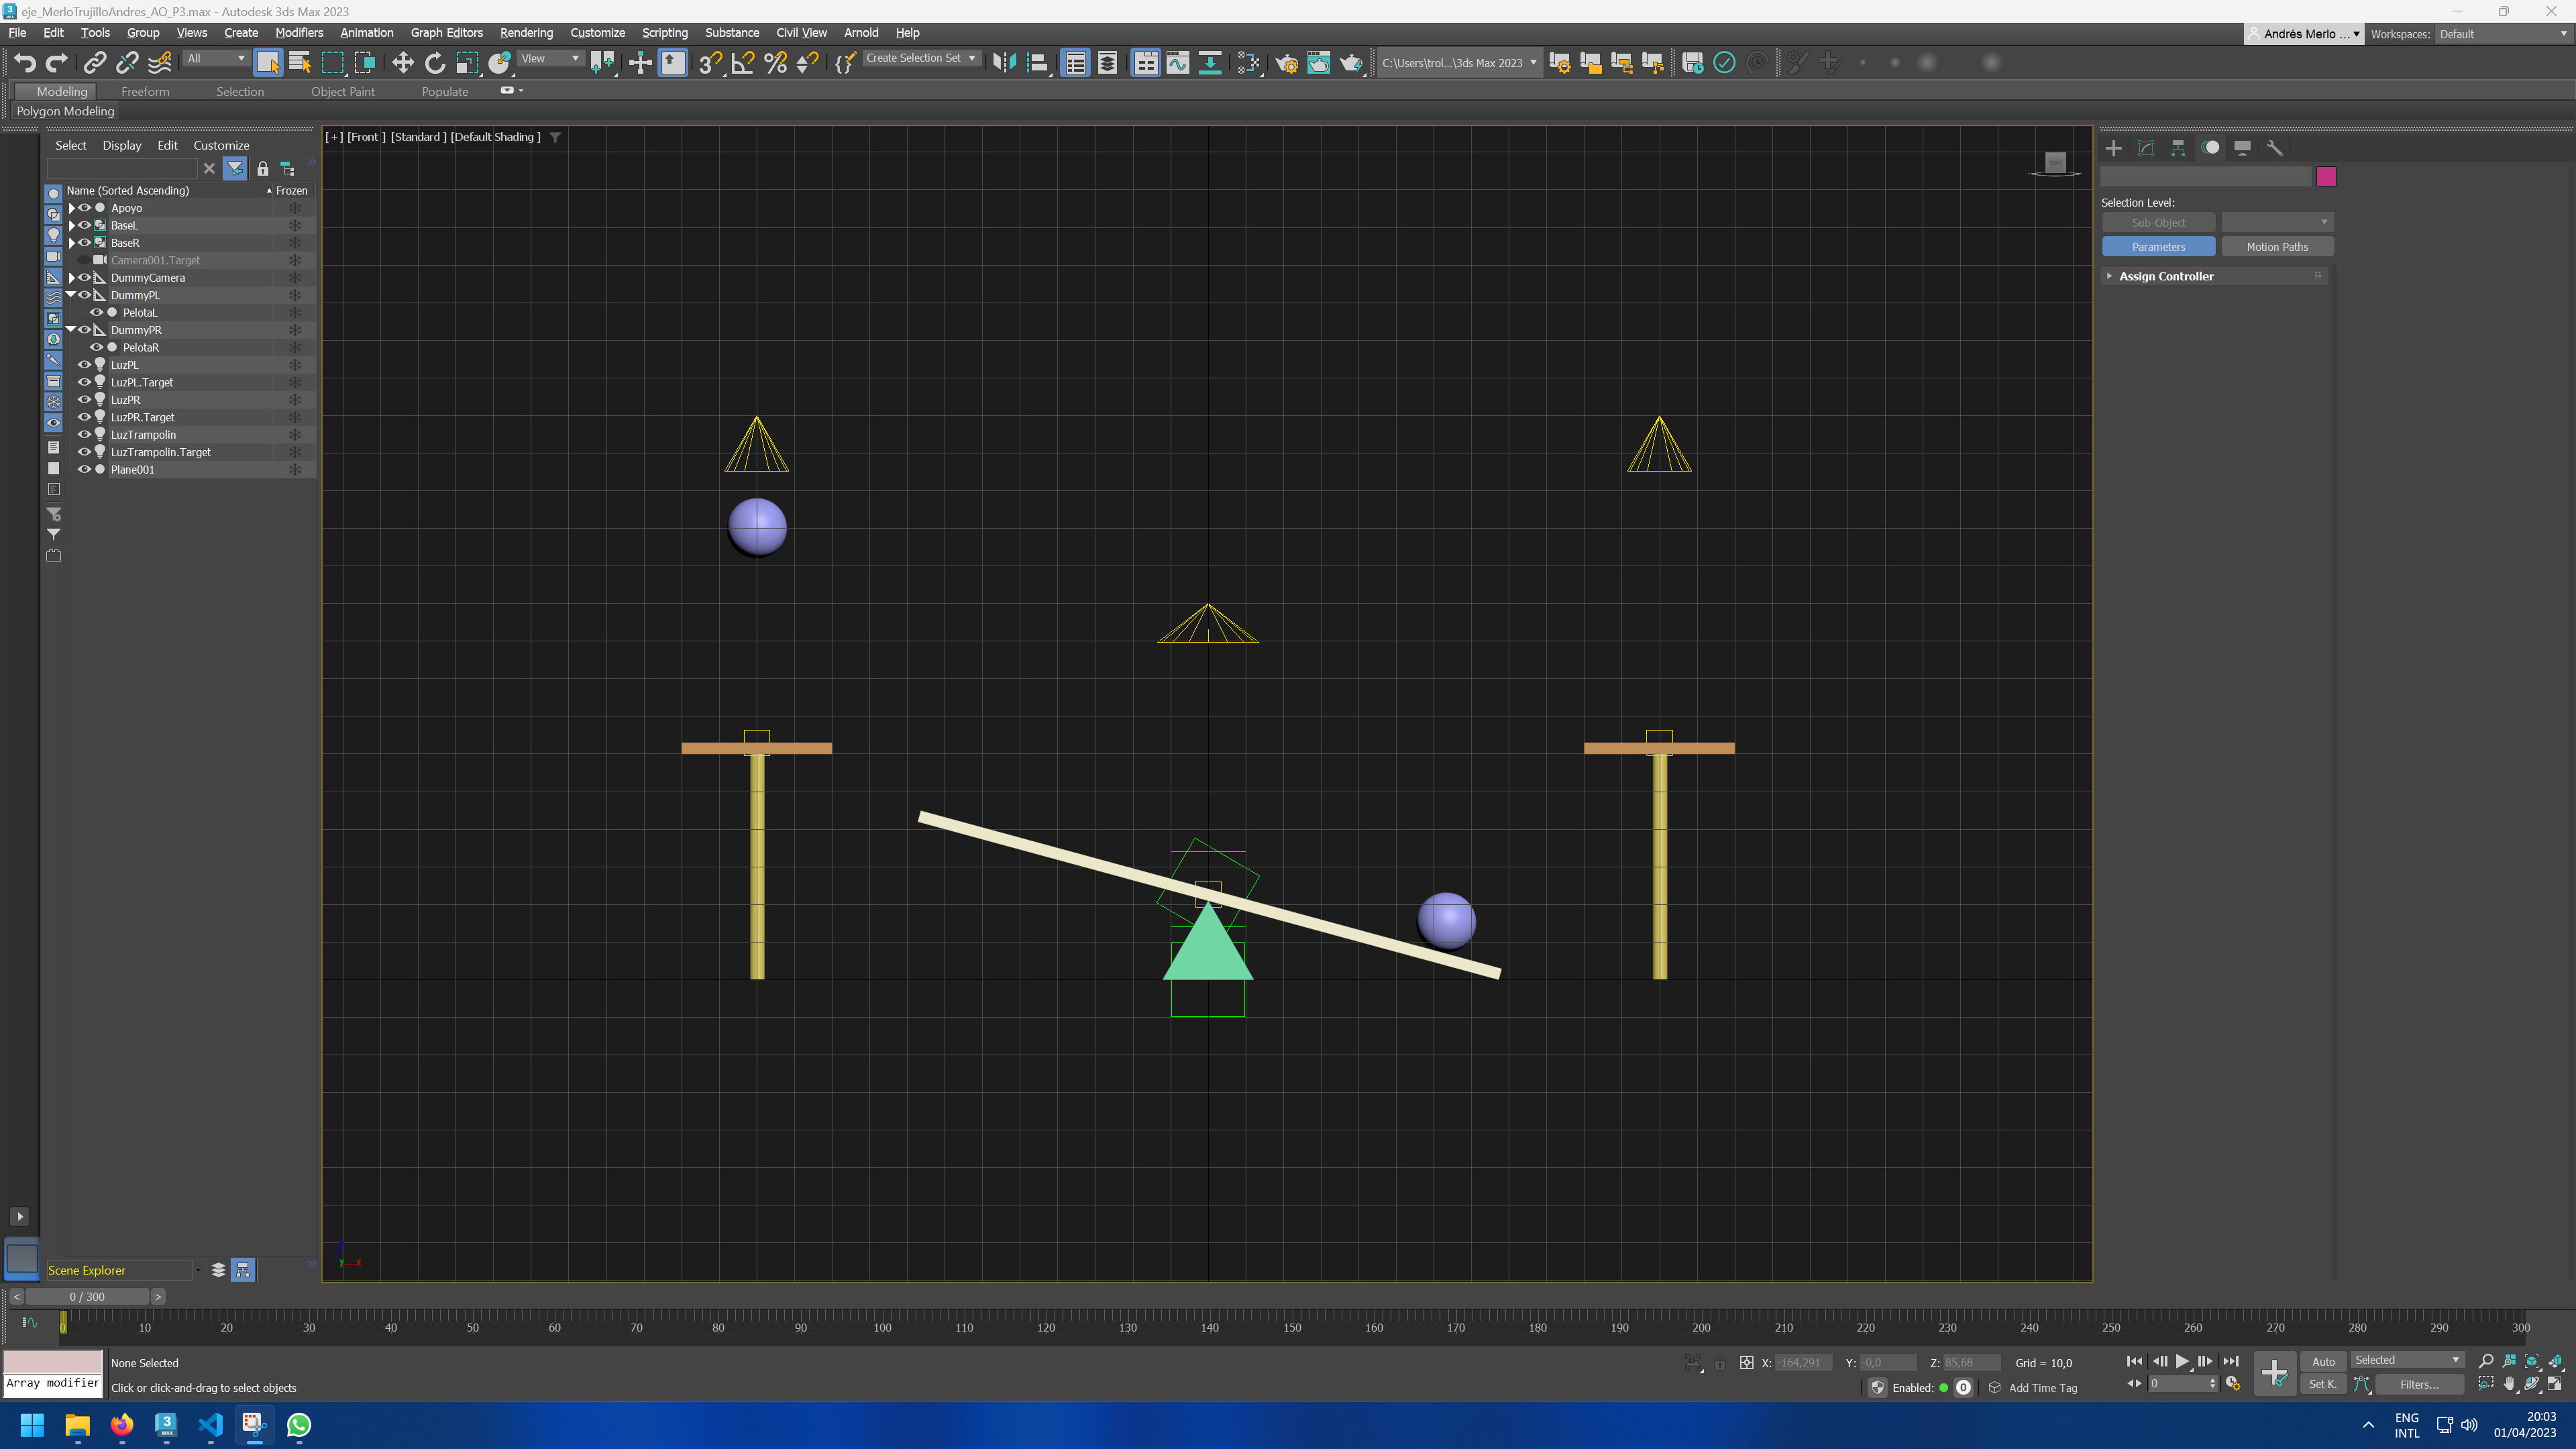
\includegraphics[width=\textwidth]{imagenes/Ejercicio 1/keyframes/0.png}
%         \caption{Pelotas en el instante 0.}
%     \end{subfigure}
%     \hfill
%     %\par\bigskip %si se desea dejar un margen entre la imagen de arriba y de abajo
% 	\begin{subfigure}[t]{0.48\textwidth}
% 	    \centering
% 	    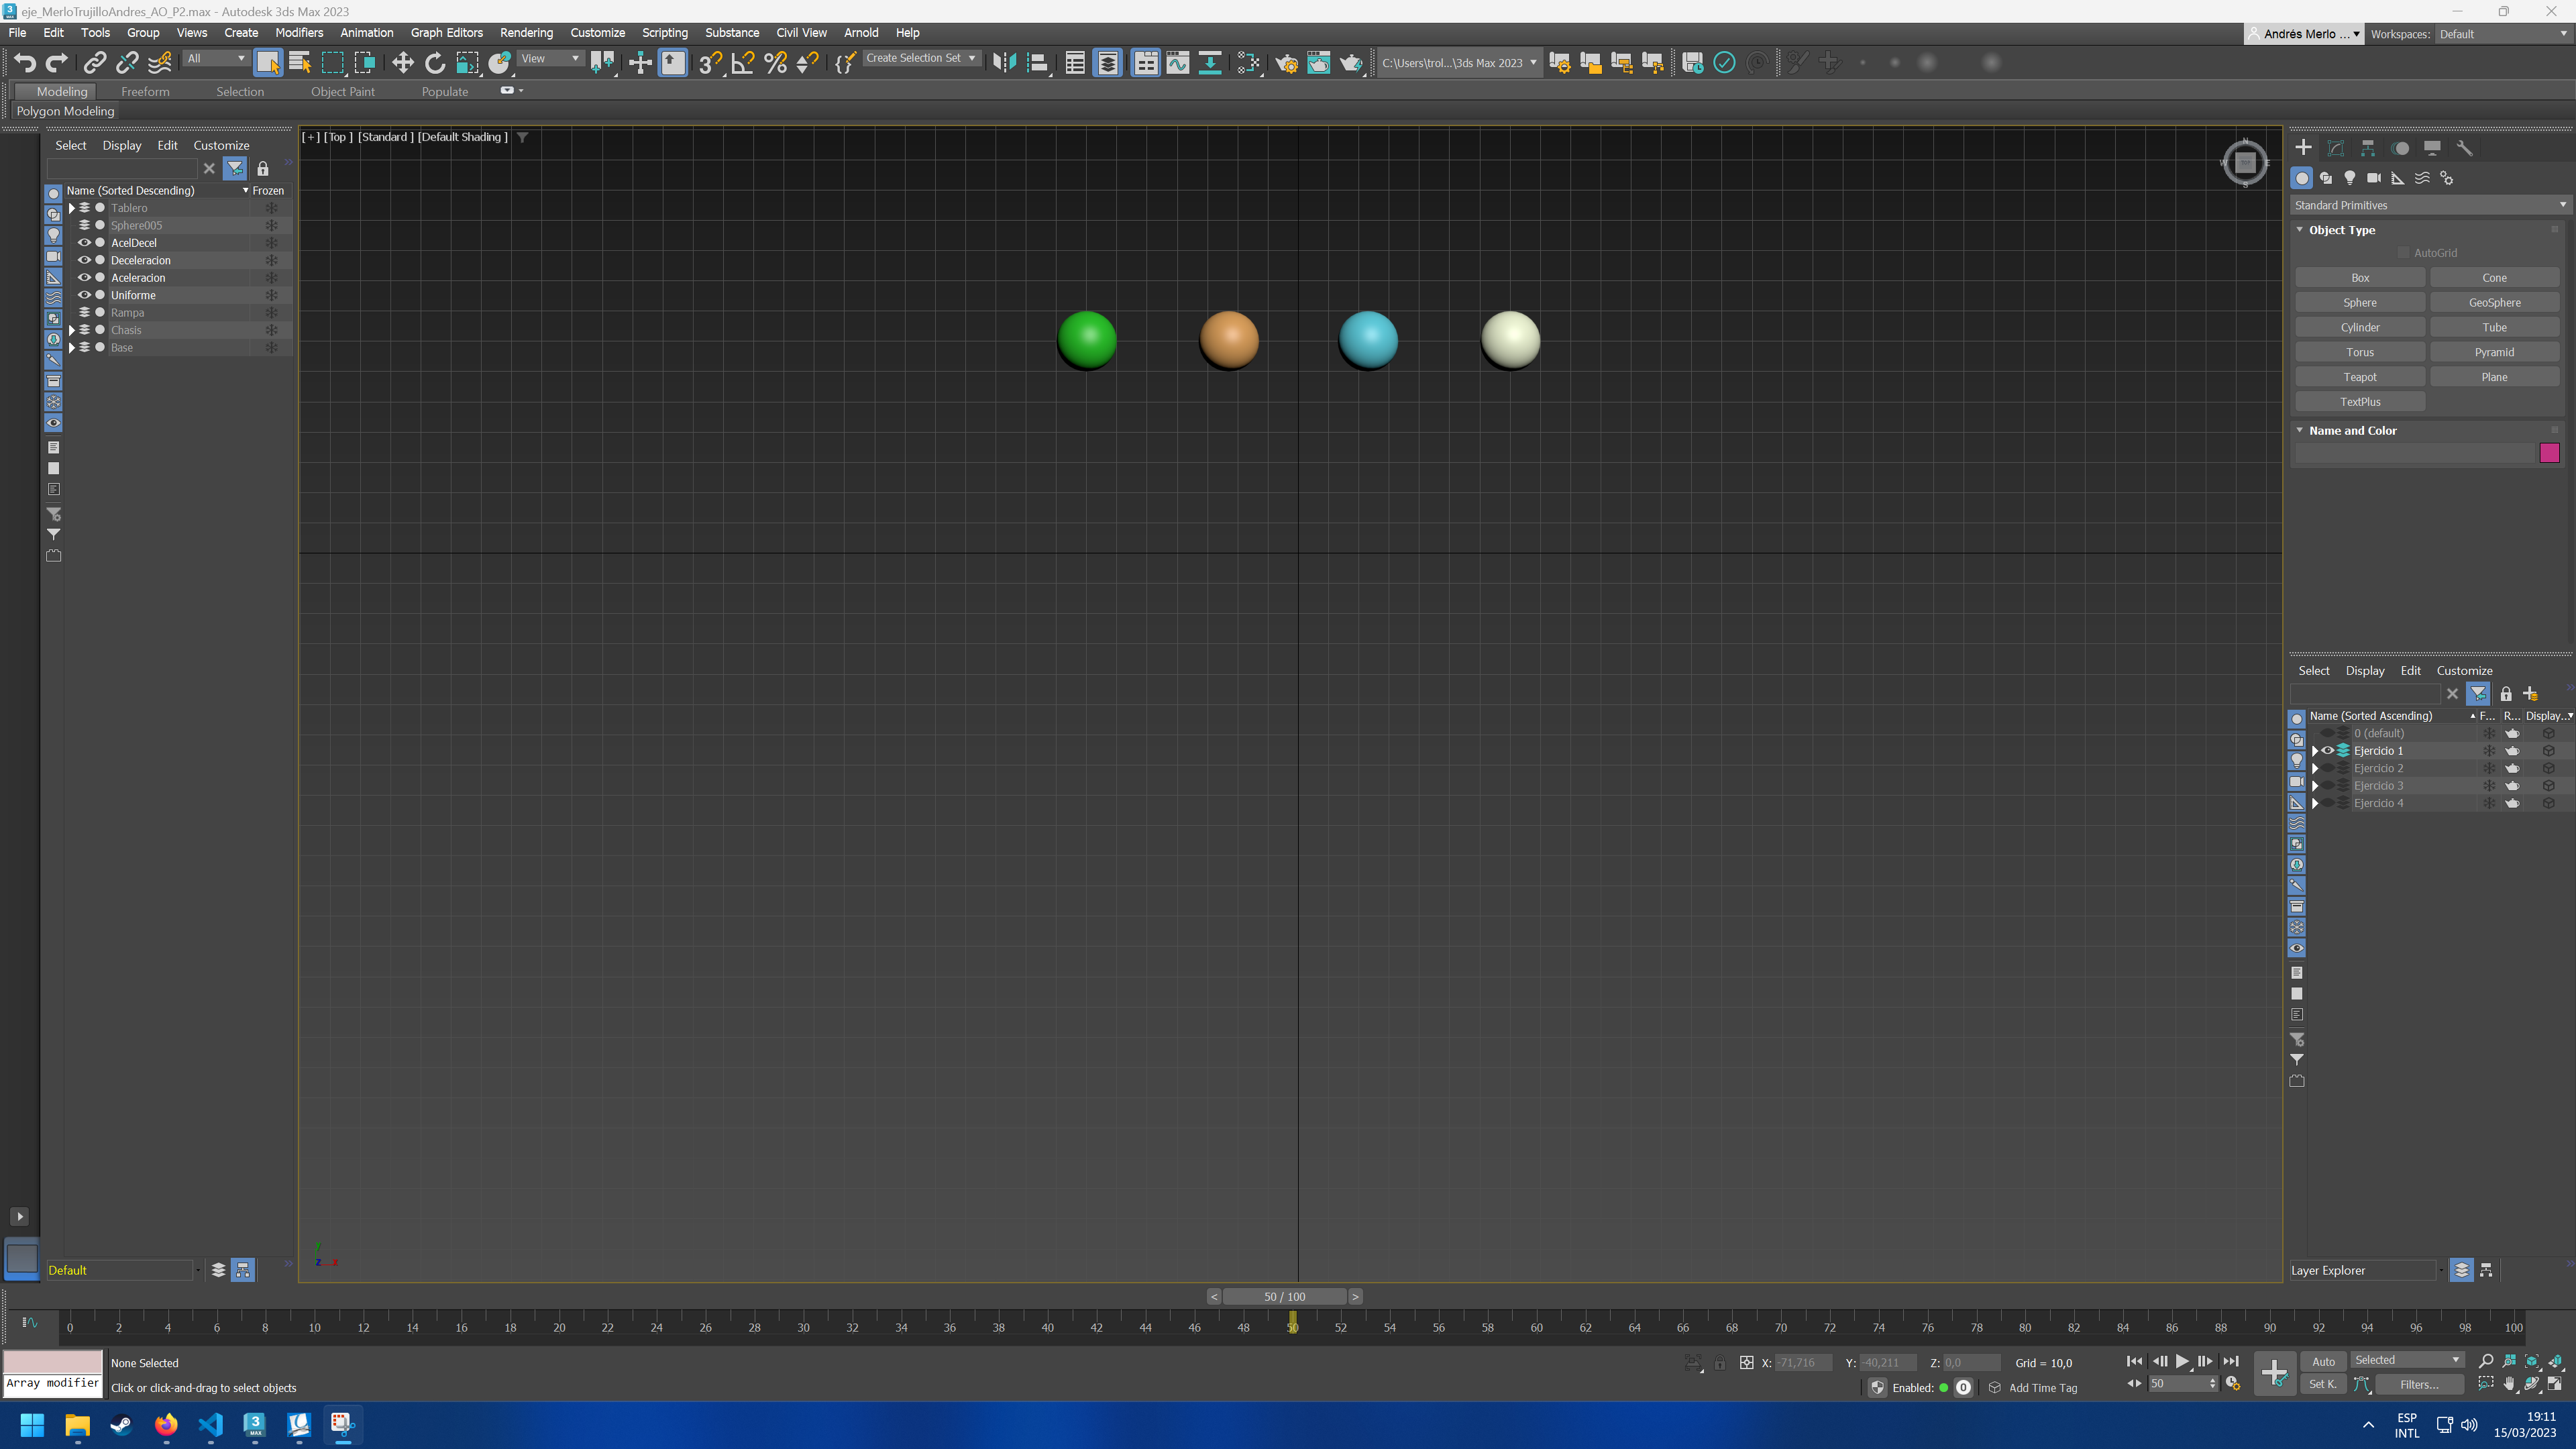
\includegraphics[width=\textwidth]{imagenes/Ejercicio 1/keyframes/50.png}
%         \caption{Pelotas en el instante 50.}
%     \end{subfigure}    
% \end{figure}

% $30 \text{fps} \times 2 \times 5 \text{segundos} = 300 \text{fotogramas} $
\section[Da algún ejemplo de objetos, o partes de objetos, con: 1 grado de libertad y 2 grados de libertad. Indica qué movimientos se permiten. Pon un ejemplo visual.]{
Da algún ejemplo de objetos, o partes de objetos, con: 
\begin{itemize}[leftmargin=3em]
   \item 1 grado de libertad.
   \item 2 grados de libertad.
\end{itemize}
\begin{quote}
   ~~Indica qué movimientos se permiten. Pon un ejemplo visual.
\end{quote}
}

Voy a dividir los objetos y la explicación con 1 y 2 grados de libertad en subsecciones distintas:

\subsection{1 grado de libertad}

Un ejemplo puede ser la bisagra de una puerta, ya que solo se permite la rotación en el eje Z (suponiendo unas coordenadas Z-Up).

\begin{figure}[H]
   \centering
   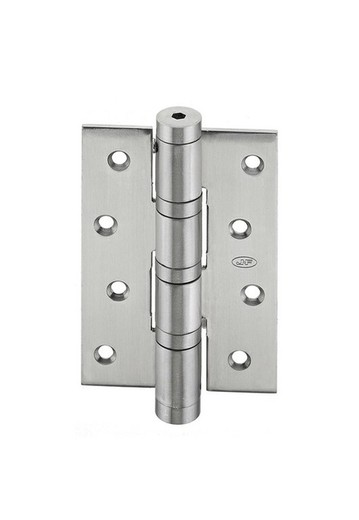
\includegraphics[width=0.3\textwidth]{imagenes/bisagra.jpeg}
   \caption{Ejemplo de una bisagra simple\cite{bisagra}.}
\end{figure}

Otro ejemplo podría ser el muelle de un vehículo, ya que solo puede ser escalado en uno de los ejes (normalmente el eje Z).

% foto del muelle y a ver si encuentro alguno de una bisagra
\begin{figure}[H]
   \centering
   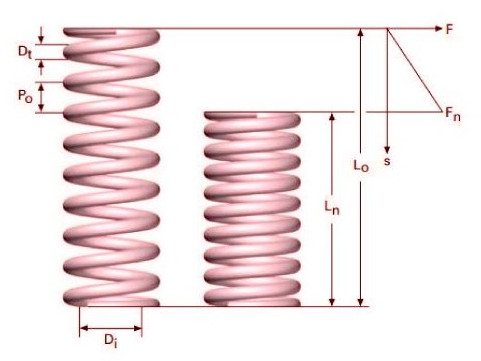
\includegraphics[width=0.5\textwidth]{imagenes/muelle.jpg}
   \caption{Ejemplo de un muelle. Se puede observar que el escalado en el eje vertical hace que se comprima\cite{muelle}.}
\end{figure}

\subsection{2 grados de libertad}

Un ejemplo claro de un objeto con dos grados de libertad es el de un joystick de videojuegos, ya que permite rotaciones hacia arriba y abajo (eje Y) y rotaciones hacia la derecha e izquierda (eje X).

% foto de calibracion joystick, quizas de la switch, que se ve mejor
\begin{figure}[H]
   \centering
   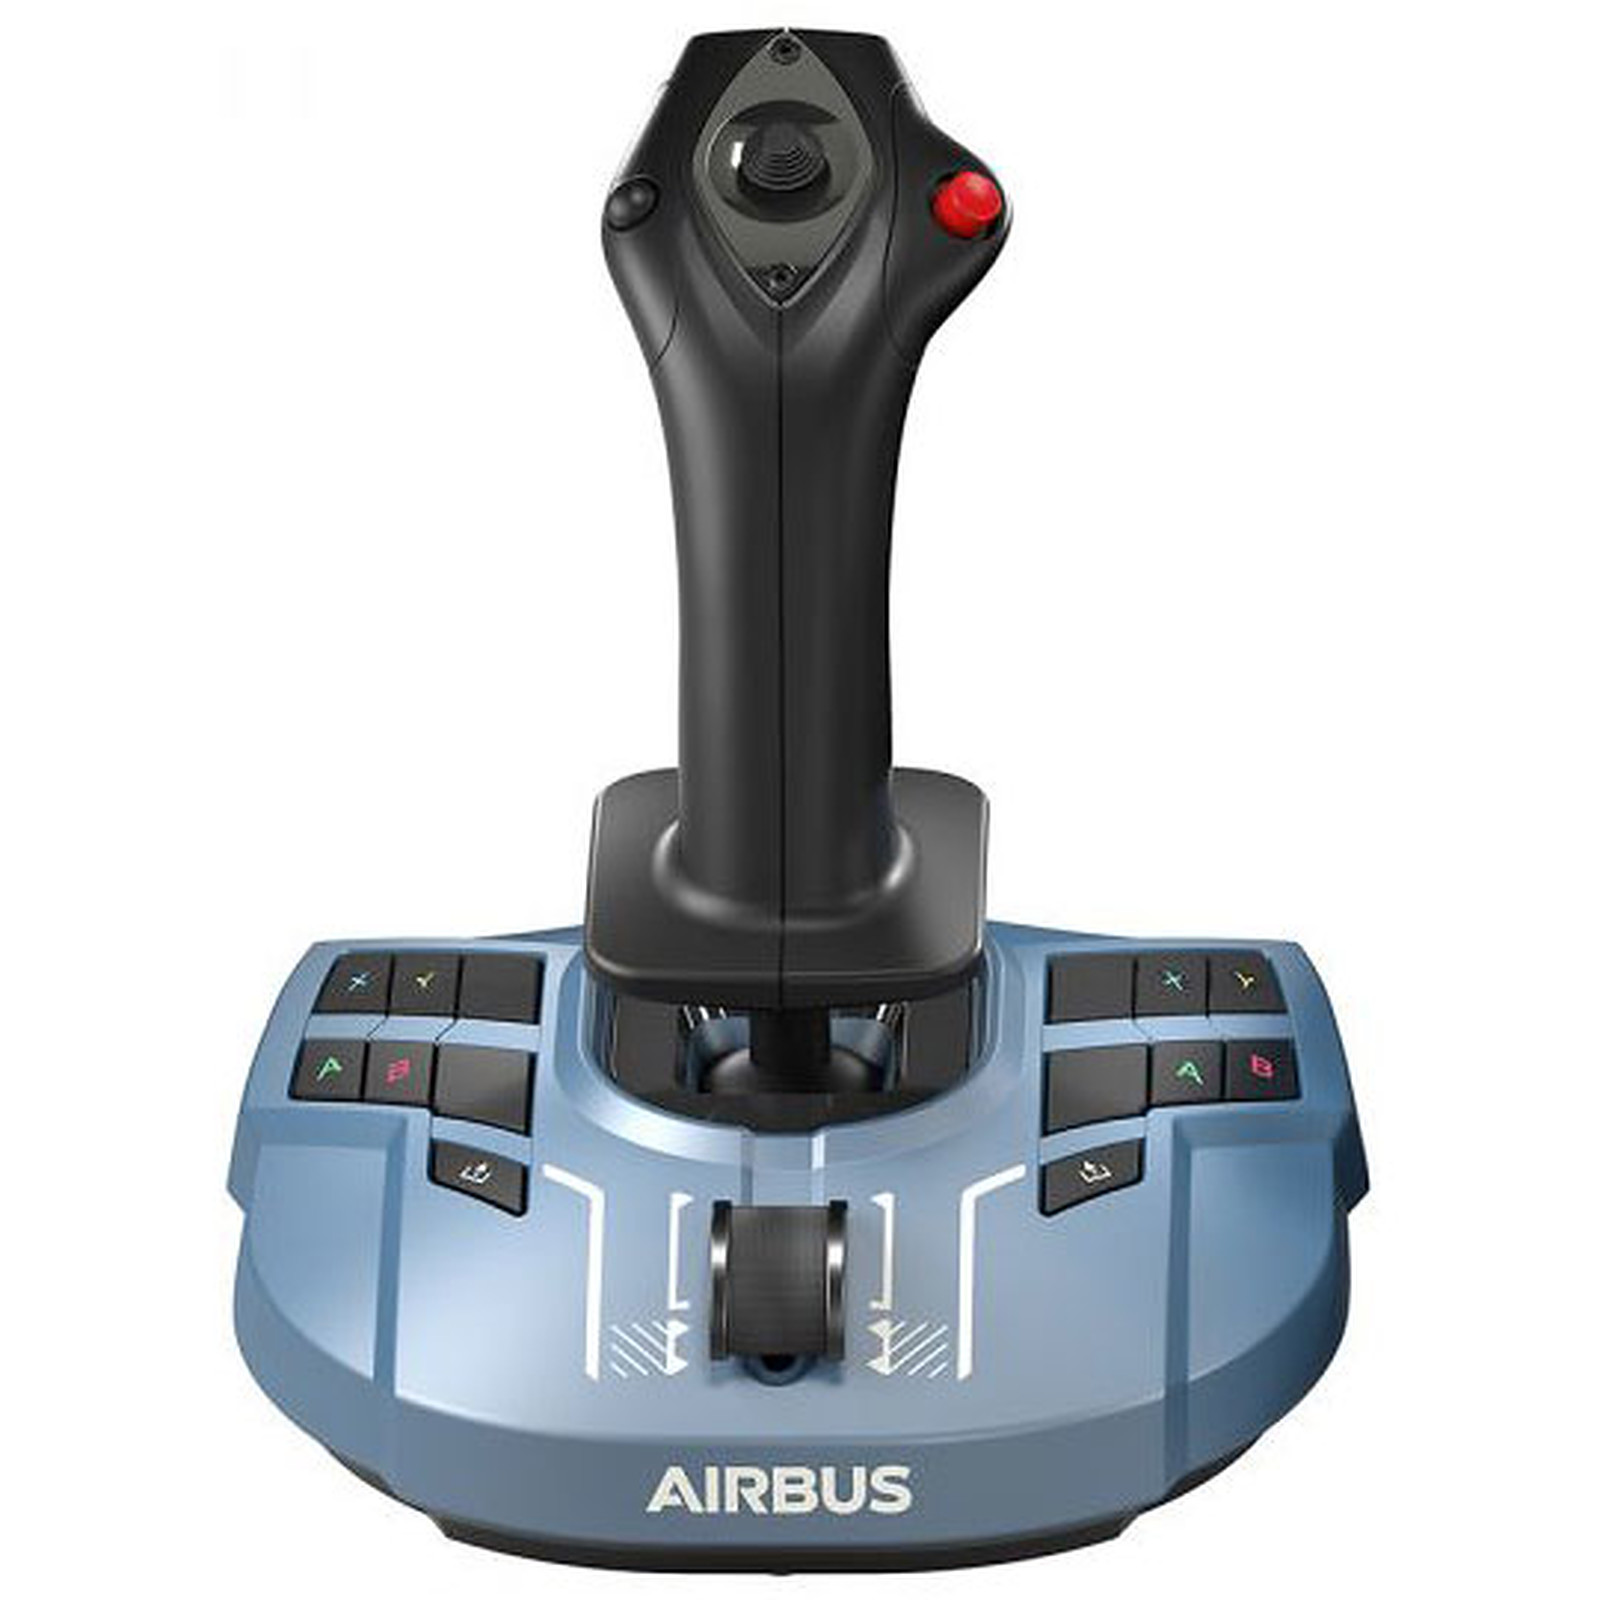
\includegraphics[width=0.5\textwidth]{imagenes/joystick.jpg}
   \caption{Joystick utilizado para simuladores de aviones. Solo permite rotaciones en dos ejes\cite{joystick}.}
\end{figure}

\section[Busca en 3DS Max la plantilla (Biped o CAT). Crea un esqueleto. Modifica alguna propiedad. Ponlo en una pose distinta a la que está por defecto.]{
   Busca en 3DS Max la plantilla (Biped o CAT).
   \begin{itemize}[leftmargin=3em]
      \item  Crea un esqueleto.
      \item Modifica alguna propiedad.
      \item Ponlo en una pose distinta a la que está por defecto.
   \end{itemize}   
}

Para crear un esqueleto es necesario acceder a los menús superiores: Create $\rightarrow$ Systems $\rightarrow$ Biped.

% foto de los menus
\begin{figure}[H]
   \centering
   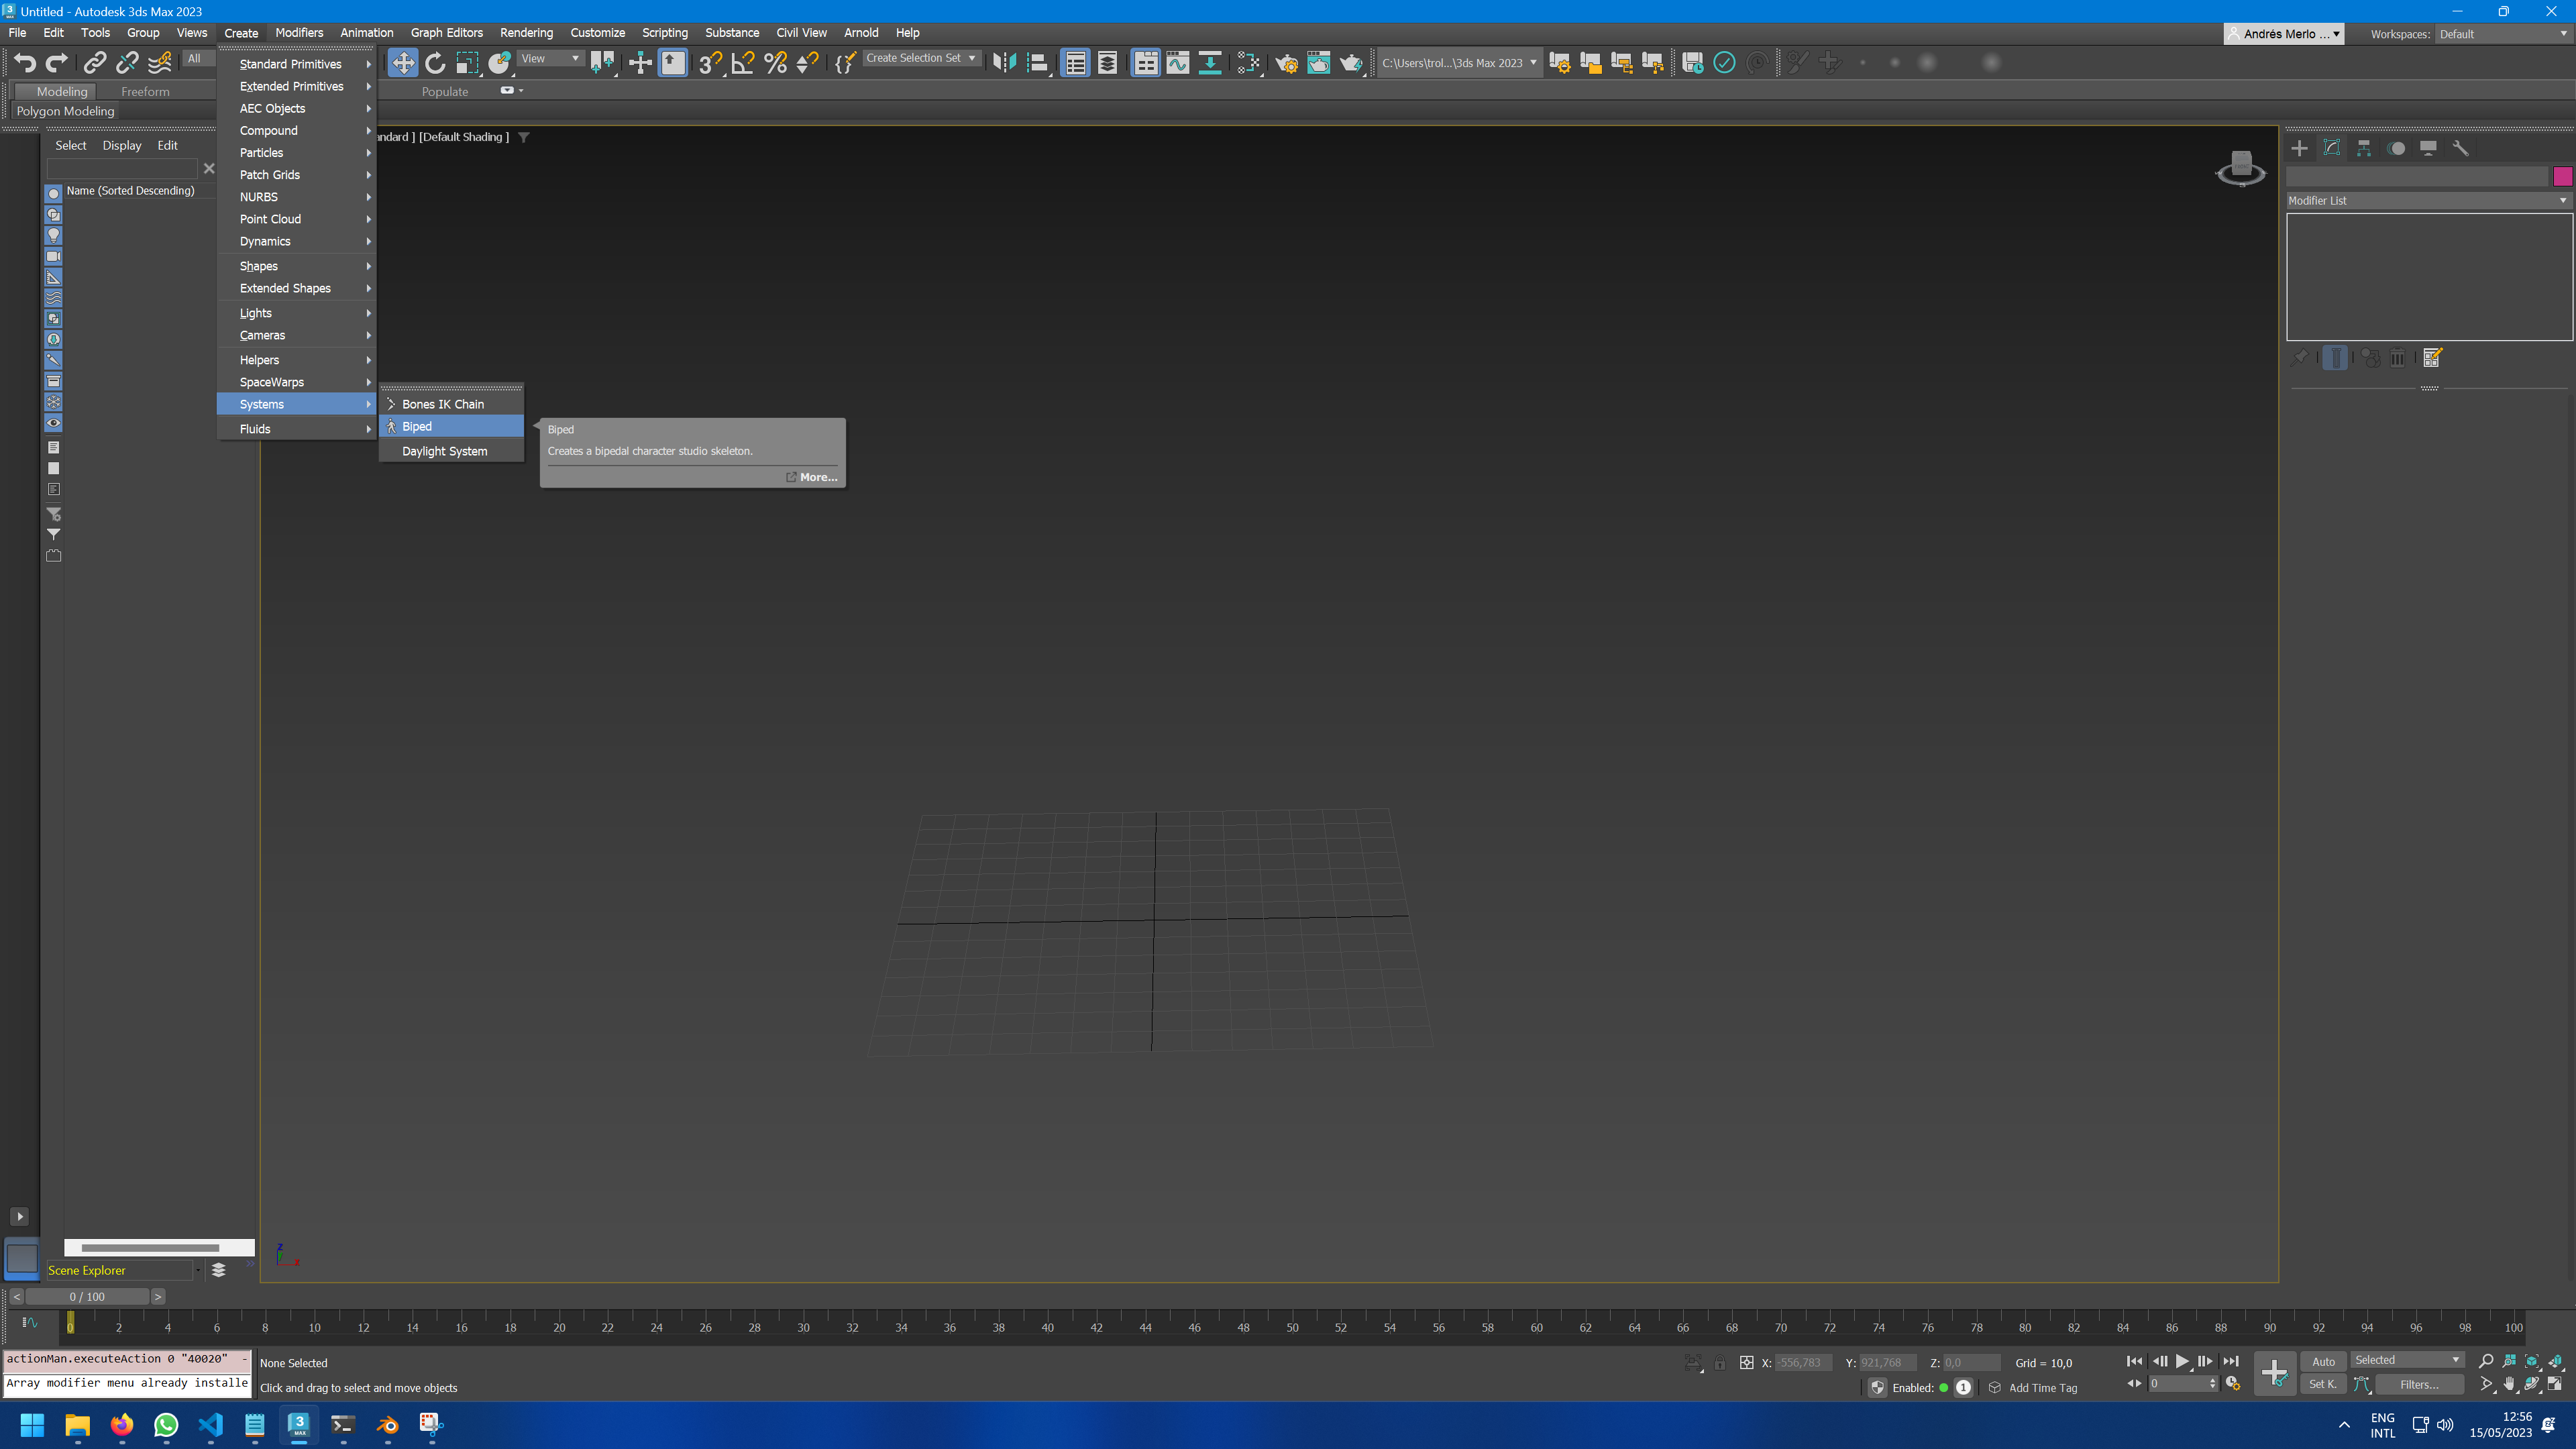
\includegraphics[width=0.7\textwidth]{imagenes/menus.png}
   \caption{Localización del Biped en los menús.}
\end{figure}

Otra forma de crear un Biped es en la sección de la derecha donde se crean los cubos y formas básicas, en la última subsección.

\begin{figure}[H]
   \centering
   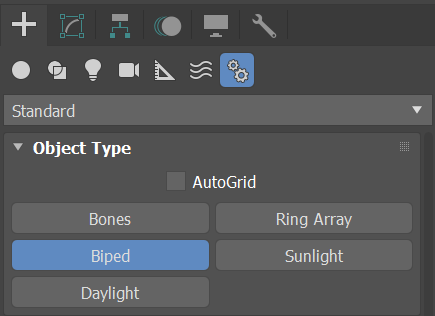
\includegraphics[width=0.5\textwidth]{imagenes/bipedNew.png}
   \caption{Localización alternativa para crear un Biped.}
\end{figure}

Además, aparece un menú para poder modificar sus propiedades, similar a otras figuras básicas:

\begin{figure}[H]
   \centering
   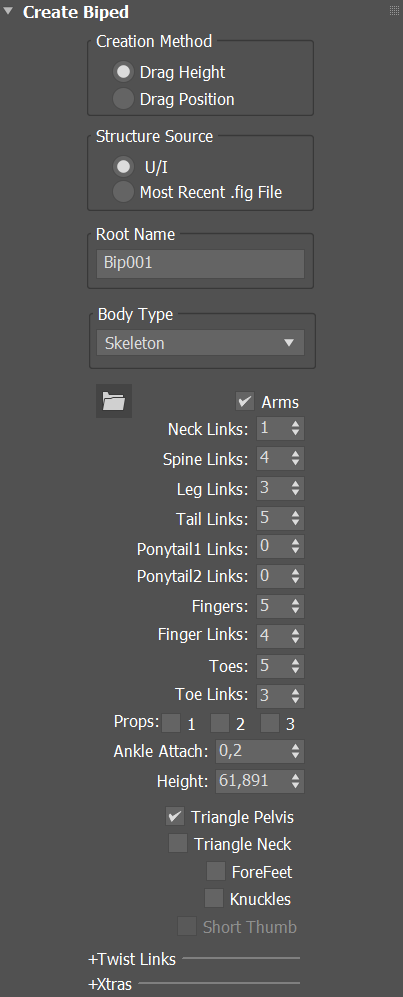
\includegraphics[width=0.3\textwidth]{imagenes/prop.png}
   \caption{Propiedades del biped.}
\end{figure}

He modificado las propiedades del biped para que tenga todos los dedos de las manos y de los pies y tenga una cola.

\bigskip
\newpage

A continuación, se pone en la escena como cualquier otro objeto.

% figura del bicho puesto
\begin{figure}[H]
   \centering
   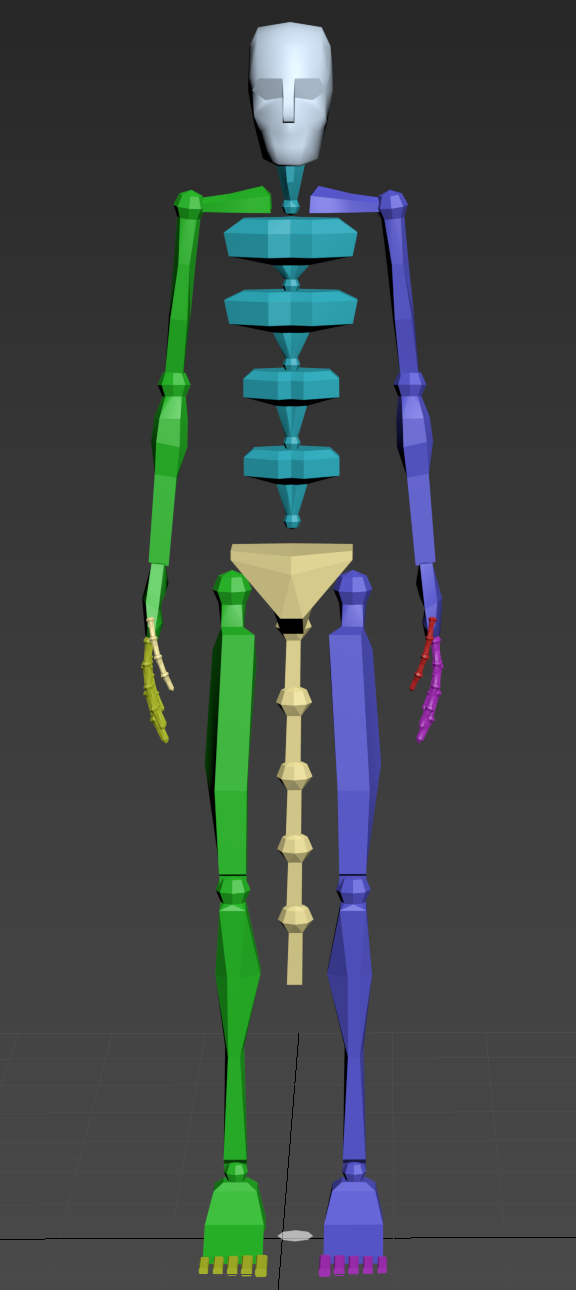
\includegraphics[width=0.25\textwidth]{imagenes/biped2.png}
   \caption{Biped generado en la escena.}
\end{figure}

Si se selecciona cualquier extremidad, se puede rotar o trasladar, realizando un movimiento similar al del cuerpo humano.

% pose distinta
\begin{figure}[H]
   \centering
   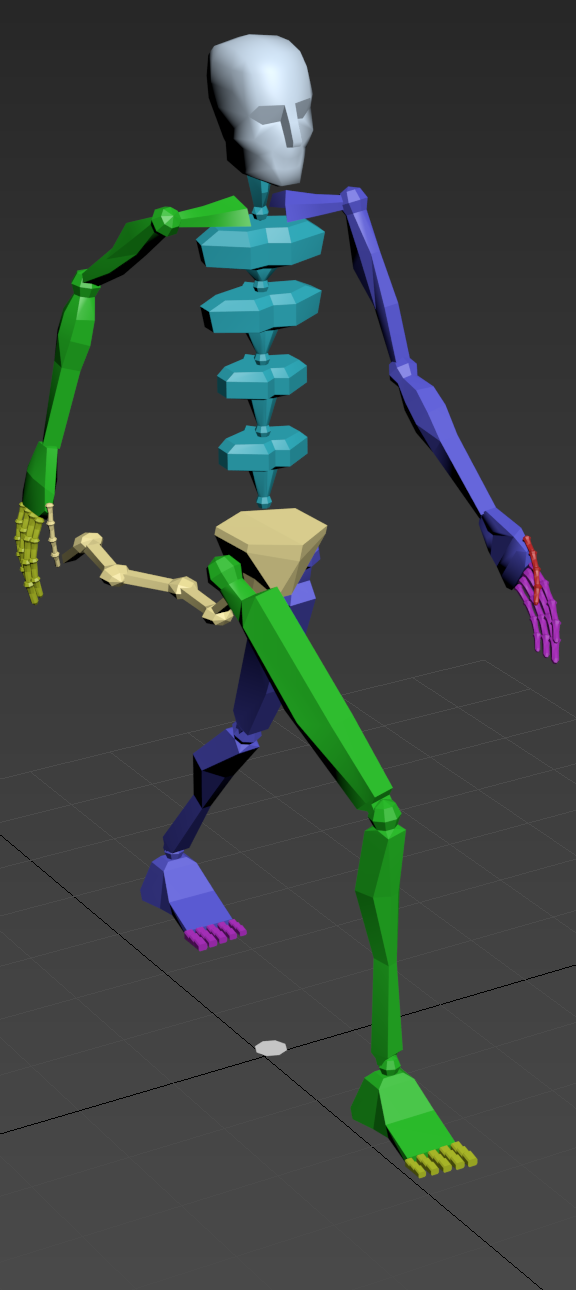
\includegraphics[width=0.25\textwidth]{imagenes/bipedWalk2.png}
   \caption{Posición del biped modificada. Simulando que está caminando y con la cola en otra posición.}
\end{figure}

\newpage

\section{Indica algún ejemplo en el que con cinemática inversa se podrían obtener múltiples soluciones.}

Un ejemplo puede ser si se desea llegar a una pose en el que el personaje se toque la nariz con el dedo, ya que la posición del codo, la rotación del hombro y la posición de los brazos puede ser más de una.

\bigskip 

Otro ejemplo similar puede ser en cualquier posición de mano en la que el codo no se encuentre extendido del todo, de forma que la posición del codo y la rotación del hombro pueda ser más de una.

\subsection{¿Se podría encontrar algún escenario donde no existe una solución con cinemática inversa?}

Sí. Se puede dar el caso en el que no haya ninguna solución. Un ejemplo es el de intentar tocar el codo con los dedos de la mano del mismo brazo, ya que es una postura que no es natural para la anatomía del cuerpo humano.

\subsection{¿Qué problemas puede tener trabajar con IK?}

El principal problema es que no se va a saber la interpolación utilizada para llegar al resultado final, dando lugar a soluciones que el animador no esperaba. Ocurre principalmente cuando la diferencia de posición entre los dos instantes es demasiado grande, haciendo que pueda ser necesario poner más fotogramas clave para asegurar una correcta interpolación.

\newpage

\section[Indica cómo se crearía un modelo con varias piezas donde: El elemento superior rote respecto del elemento que hace de juntura. La rotación de este elemento implica la rotación de los inferiores en menor grado cuanto más se aleja del primero.]{
   Indica cómo se crearía un modelo con varias piezas donde:
   \begin{itemize}[leftmargin=3em]
      \item El elemento superior rote respecto del elemento que hace de juntura.
      \item La rotación de este elemento implica la rotación de los inferiores en menor grado cuanto más se aleja del primero.
   \end{itemize}
}

\begin{figure}[H]
   \centering
   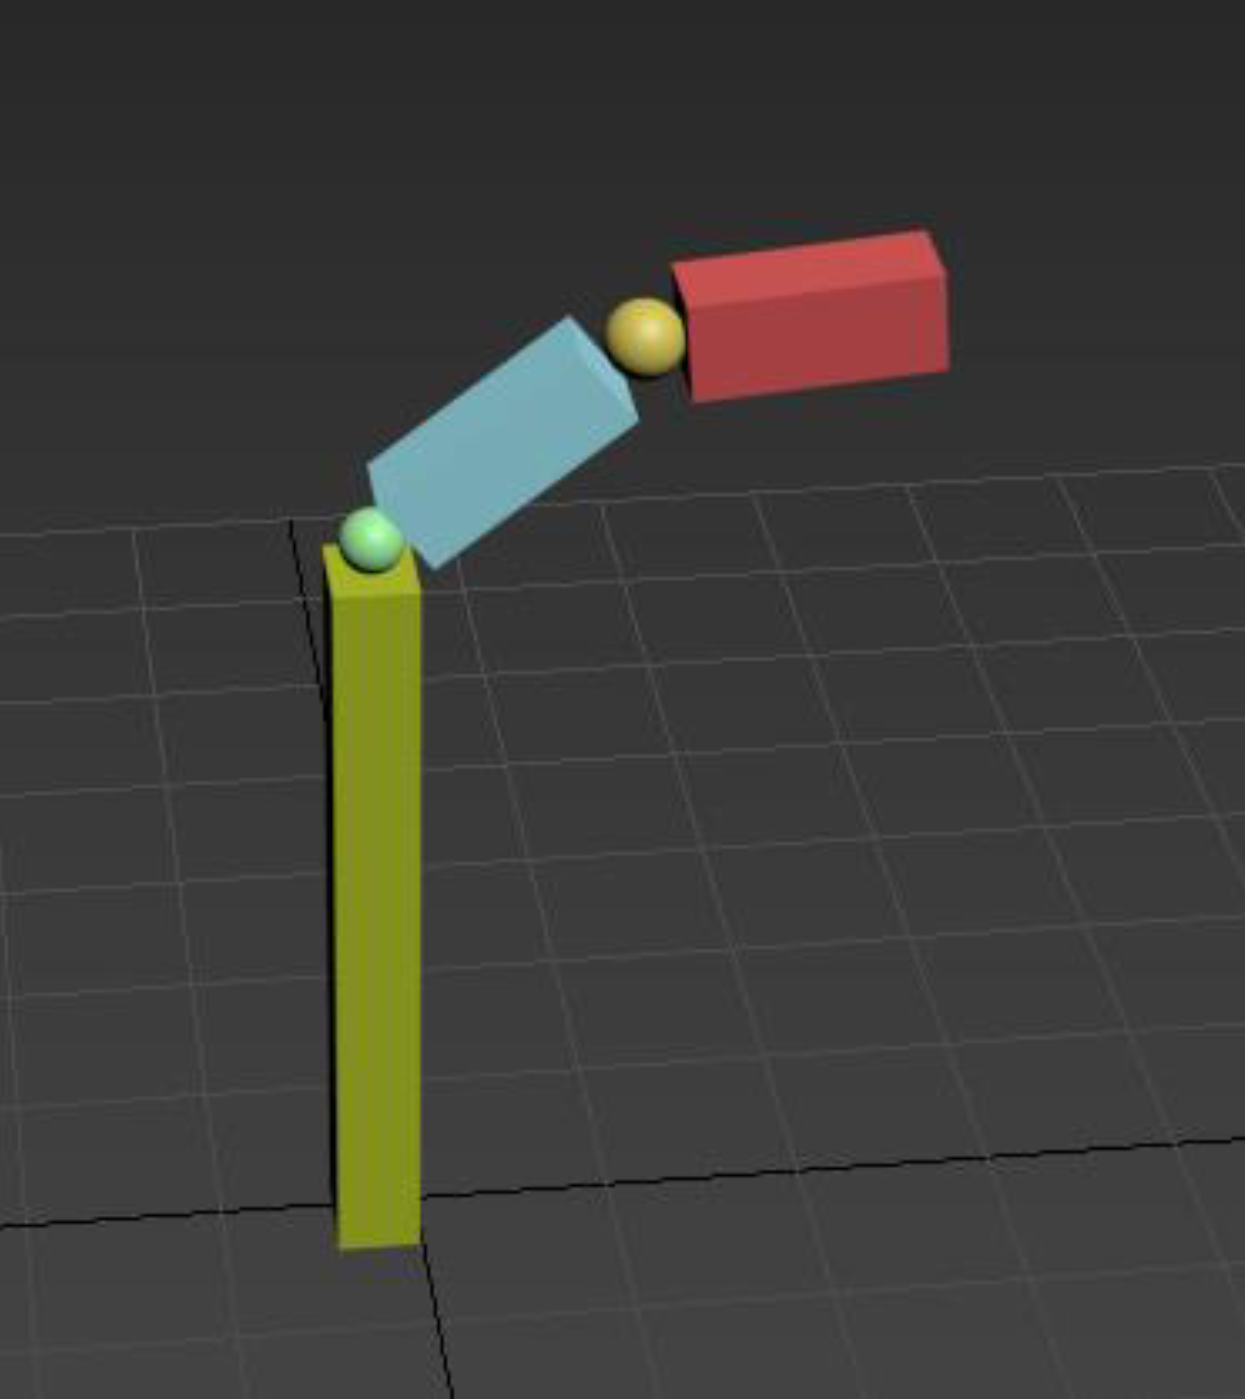
\includegraphics[width=0.3\textwidth]{imagenes/pag42.png}
   \caption{Imagen del enunciado\cite{diapos}.}
\end{figure}

Lo primero que hay que hacer es crear la jerarquía de las piezas, de forma que el cubo verde sea padre del azul y este a su vez del rojo. Después, se rotan las esferas para que el objeto se encuentre en la misma postura que la del enunciado.

% foto jerarquia
\begin{figure}[H]
   \centering
   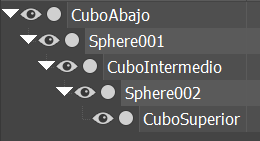
\includegraphics[width=0.3\textwidth]{imagenes/jerarquia.png}
   \caption{Jerarquía utilizada para el brazo.}
\end{figure}

A continuación, para que el giro del cubo rojo se vea reflejado en los demás, es necesario utilizar \textit{Wire Parameter} en la rotación del eje Z y hace falta aplicarle un factor de reducción para que los cubos azul y verde vayan más lentos. En mi caso, el factor de reducción ha sido de 2, de forma que el cubo de más arriba le aporta la mitad de rotación al intermedio, y el intermedio le aporta la mitad de rotación al de abajo, haciendo que sea 0.25 con respecto al superior.

\bigskip
\newpage

La figura final es:

\begin{figure}[H]
   \centering
   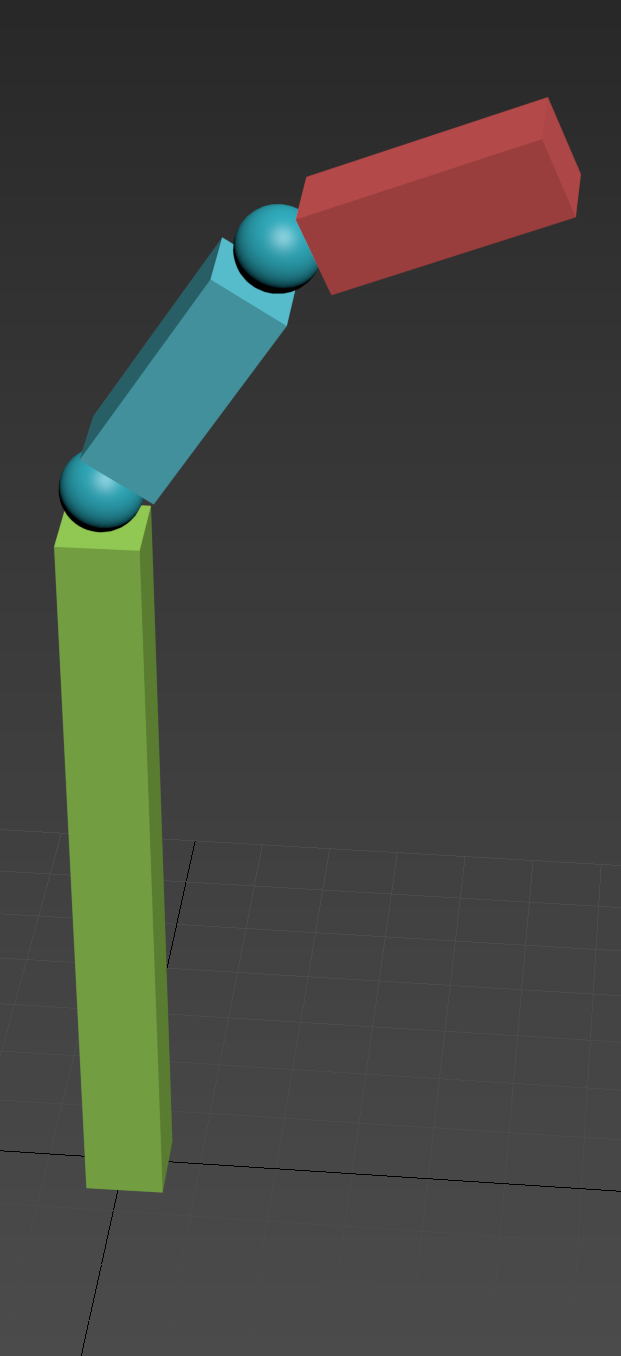
\includegraphics[width=0.3\textwidth]{imagenes/brazo1mio.png}
   \caption{Brazo del ejercicio modelado.}
\end{figure}

Y si le aplico una rotación, se puede ver que las piezas de abajo rotan menos:

\begin{figure}[H]
   \centering
   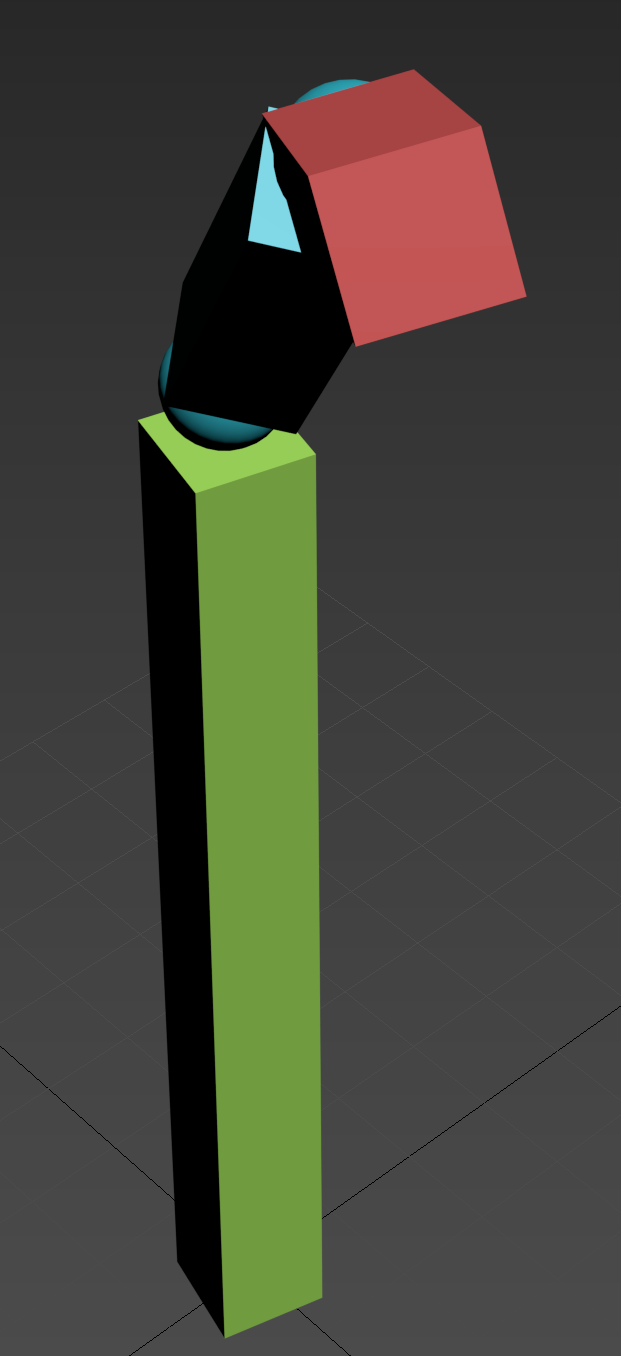
\includegraphics[width=0.3\textwidth]{imagenes/brazo2mio.png}
   \caption{Rotación de la figura en el eje X.}
\end{figure}

\newpage

\section[¿Qué es preferible? Crear un modelo con el mayor número posible de grados de libertad, es decir un rigging completo. Crear un modelo con el menor número de grados de libertad, un rigging minimalista. Justifica la respuesta.]{
   ¿Qué es preferible?
   \begin{itemize}[leftmargin=3em]
      \item Crear un modelo con el mayor número posible de grados de libertad, es decir un rigging completo.
      \item Crear un modelo con el menor número de grados de libertad, un rigging minimalista.
   \end{itemize}
   \begin{quote}
      ~~Justifica la respuesta.
   \end{quote}
}

% rescribir
Depende del contexto. Por ejemplo, si va a haber una toma en la que se vea de cerca a un personaje o una extremidad como las manos, lo más aconsejable es utilizar un rigging completo, con los dedos de las manos incluidos. En cambio, si es una toma de lejos de personas caminando o animales, no es necesario utilizar un rigging tan complejo y se podría prescindir de partes como la articulación del tobillo, las manos o incluso las distintas secciones de la columna, y en el caso de los animales, se podría prescindir de la cola. Así se consigue ahorrar tiempo en animación, al no ser apreciable desde lejos los detalles.

\section{¿Qué sucedería si los vértices de una malla solamente estuvieran influenciados por un único hueso? Da un ejemplo visual.}

Podría dar lugar a deformaciones de los vértices de la malla poco realistas y a movimientos muy robóticos, ya que los huesos le aportan flexibilidad al personaje y los pesos influencian a la modificación de los vértices que no se encuentran directamente asociados al hueso, dando así más naturalidad a la animación.
% de la malla en cierta medida para dar más naturalidad. 

\bigskip

Por tanto, respondiendo a la pregunta, se daría el caso en el que algunos vértices que deberían estar influenciados por otros huesos no lo están, dando como resultado deformaciones incorrectas. En la página 34 de las transparencias aparece el siguiente ejemplo:


\begin{figure}[H]
   \centering
   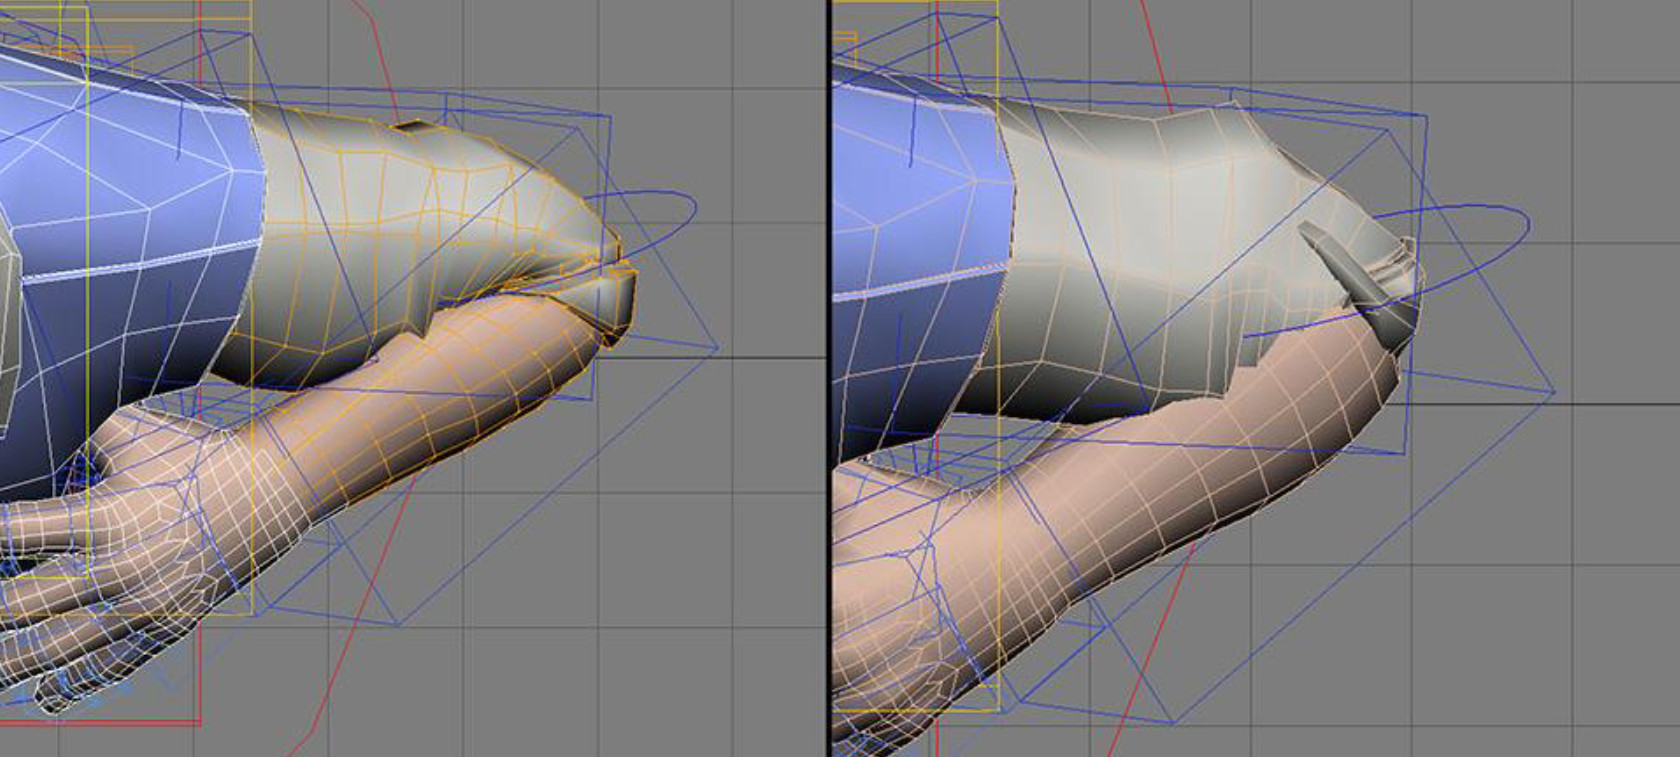
\includegraphics[width=0.7\textwidth]{imagenes/pag34.jpg}
   \caption{Animación de un brazo utilizando rigging\cite{diapos}.}
\end{figure}

Como se puede ver en la imagen de la derecha, la manga de la camiseta se deforma de manera incorrecta, dando como resultado solapamientos con la propia camiseta y los músculos del antebrazo no se comprimen debido a la compresión con el brazo.

\bigskip
\newpage

A continuación, muestro otro ejemplo de rigging en Blender, donde he puesto un cilindro con un solo hueso y otro con dos, simulando un brazo.

\begin{figure}[H]
\begin{subfigure}{0.48\textwidth}
   \centering
   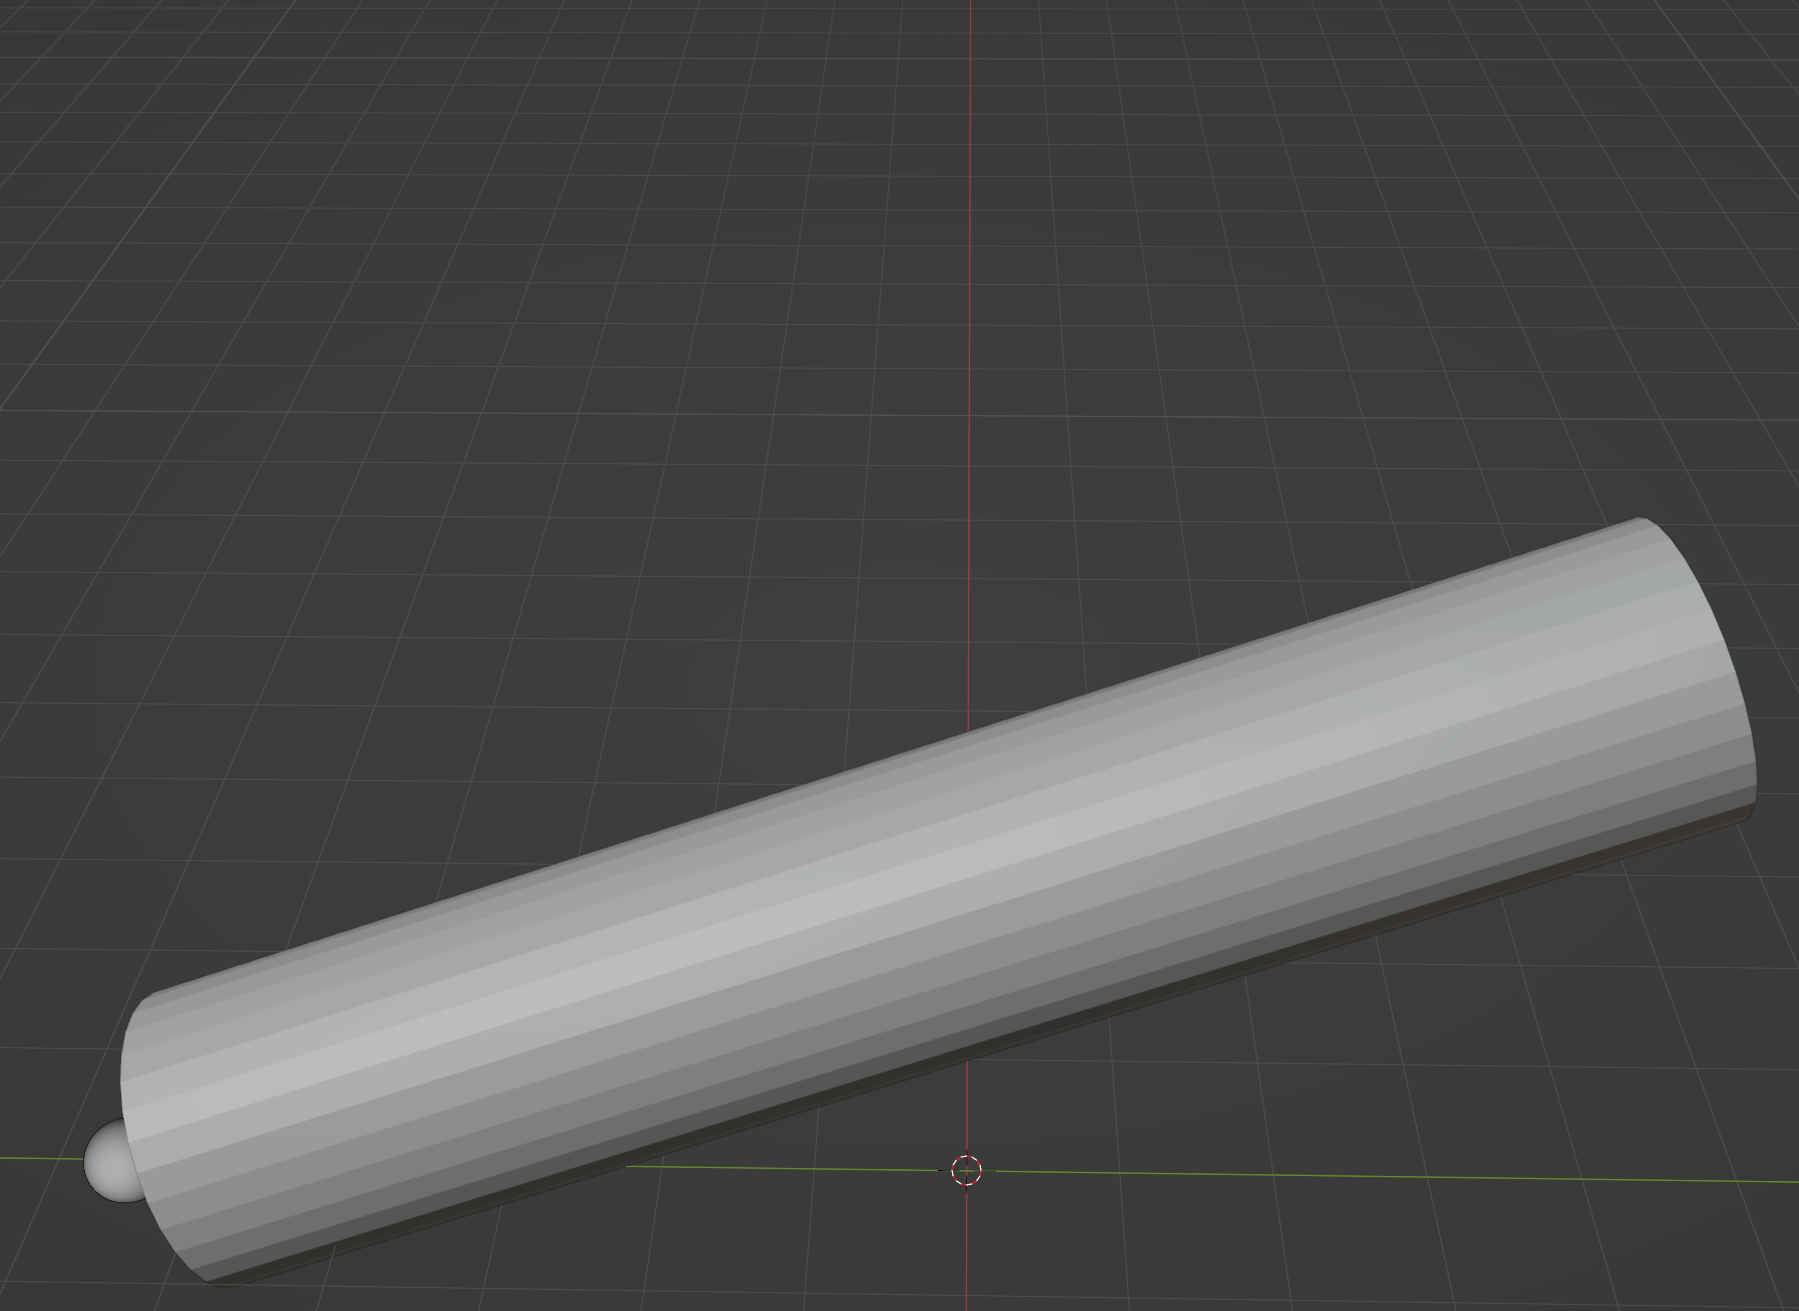
\includegraphics[width=\textwidth]{imagenes/brazo1.png}
   \caption{Cilindro con solo 1 hueso.}
\end{subfigure}
\hfill
\begin{subfigure}{0.48\textwidth}
   \centering
   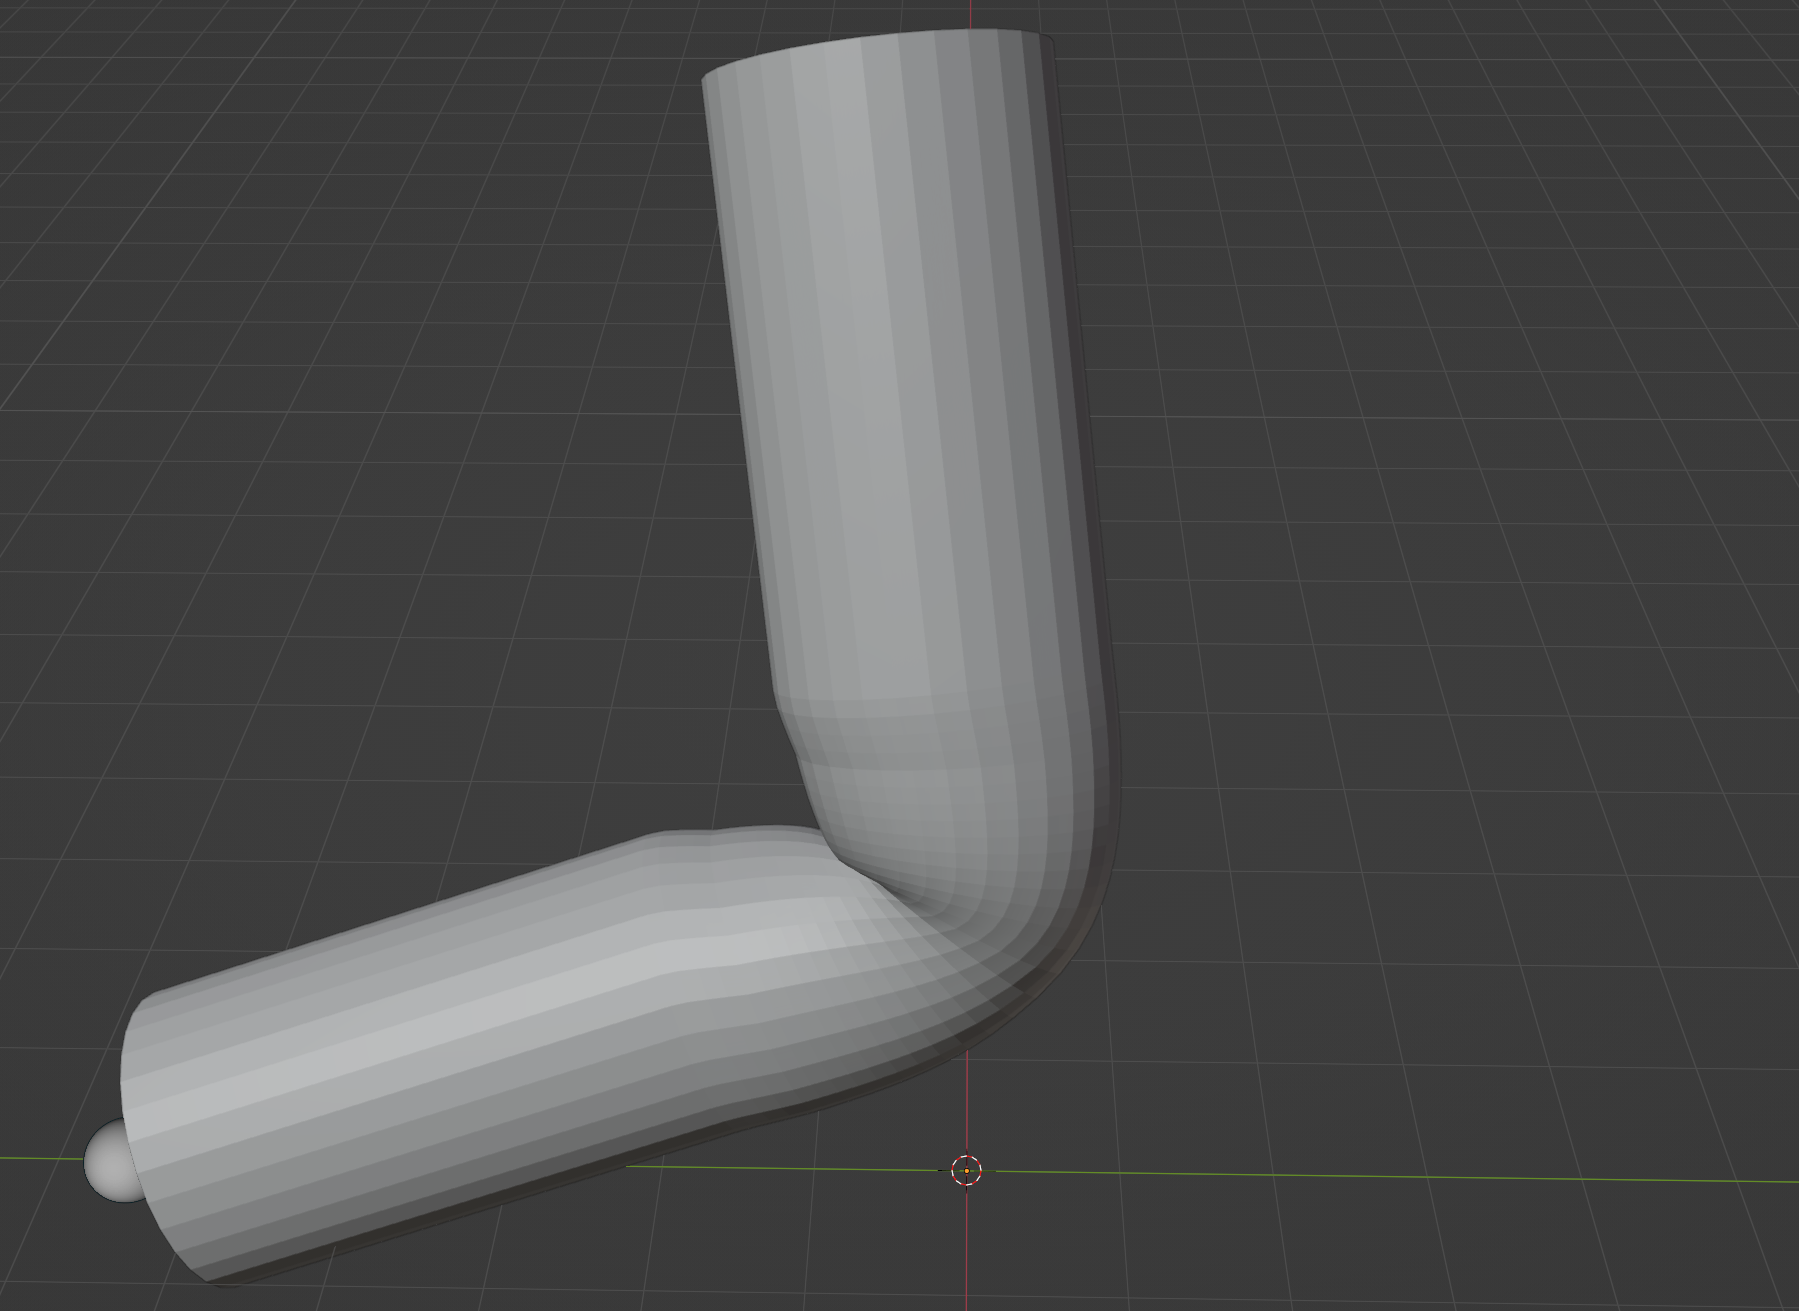
\includegraphics[width=\textwidth]{imagenes/brazo2.png}
   \caption{Cilindro con 2 huesos.}
\end{subfigure}
\end{figure}

Como se puede observar, el cilindro que solo tiene un hueso no simula de manera realista un brazo, al no poder modificar los vértices correspondientes al antebrazo (la parte de más a la derecha). Mientras que en la versión con dos huesos, es posible doblar el codo y se deforman los vértices de manera acorde a ambos pesos. Esto se puede ver mirando la cara interior del ``brazo'', donde el cilindro ha sido aplastado un poco más para que no ocurra solapamiento.

\newpage

\bibliography{bibliografia}
\bibliographystyle{plainurl}
\end{document}
